\documentclass{article}
\usepackage{graphicx}
\usepackage{hyperref}

\title{Discrete Assignment}

\begin{document}
\section*{Discrete Assignment}
\textit{ee23btech11215,Penmetsa Srikar Varma,IC Design and Technology}
\subsection*{Question 2 Exercise 5.4 chapter 5: Arithmetic Progressions of class 10}
\textbf{Q2)} The sum of the third and the seventh terms of an AP is 6 and their product is 8. Find the sum of first sixteen terms of the AP\\
\\ \textbf{Answer:\\}
Let us assume the first term of given arithmetic progression be $a(0)$ and common difference be '\textit{d}'\\
\\Let the terms of \textit{AP} be:
$$a(0),a(1),a(2)...a(k-1)$$
\textbf{Input Table:}\\
\begin{center}
\begin{tabular}{|c|c|}  
\hline
     Input Variables & Input Condition \\
\hline
     $a(2)$ & third term of \textit{AP}\\
\hline
     $a(6)$ & seventh term of \textit{AP}\\
\hline
     $a(2)$+$a(6)$ & 6 \\
\hline
     $a(2).a(6)$ & 8 \\
\hline
     $S(16)$ & sum of first 16 terms of \textit{AP}\\
\hline
\end{tabular}
\end{center}
from above we can observe that $n^{th}$ term of \textit{AP} and sum of first $n$ terms of \textit{AP} are :
\begin{equation}
\label{a1}
a(n-1)\quad and\quad S(n)
\end{equation}
then general term $a(n)$ of arithmetic progression is given by:
\begin{equation}
\label{a2}
a(n)=a(0)+n.d
\end{equation}
So from the given information the third term and seventh term of arithmetic progression be $a(2)$ and $a(6)$ respectively,
Then from (\ref{a2}):
\begin{equation}
\label{a3}
a(2) = a(0)+2d
\end{equation}
\begin{equation}
\label{a4}
a(6) = a(0)+6d
\end{equation} 
Then from (\ref{a3}) and (\ref{a4})
\begin{equation}
\label{a5}
a(2)+a(6)=6
\end{equation}
\begin{equation}
\label{a6}
a(2).a(6)=8
\end{equation}
or we can say from (\ref{a5}),
\[2a(0)+8d=6\]
\[a(0)+4d=3\]
\begin{equation}
\label{a7}
a(0)=3-4d
\end{equation}
or we can say from (\ref{a6}),
$$(a(0)+2d)(a(0)+6d)=8$$
and from (\ref{a7}),
\[(3-2d).(3+2d)=8\]
\[9-4d^2=8\]
\[d^2=\frac{1}{4}\]
\begin{equation}
\label{a8}
d=\frac{1}{2},-\frac{1}{2}
\end{equation}
Then from (\ref{a7}),
\begin{equation}
\label{a9}
a(0)=1,5
\end{equation}
We know that the sum of first \textit{n} terms of arithmetic progression is given by:
\begin{equation}
\label{a10}
S(n)= \frac{n}{2}(2.a(0)+(n-1)d)
\end{equation}
Then from (\ref{a10}) let sum of first 16 terms of arithmetic progression be $S_{16}$:
\begin{equation}
\label{general9}
S(16)= \frac{16}{2}(2a(0)+15d)
\end{equation}
Hence from (\ref{general9}),
for $a(0)$=1,d=$\frac{1}{2}$
$$S(16)=76$$
or from (\ref{general9}),
for $a(0)$=5,d=-$\frac{1}{2}$
$$S(16)=20$$
The general term of \textit{AP} ($a_n$) and sum of first \textit{n} terms of \textit{AP} ($S_n$) are given by:
$$a(n)=a(0)+n.d\quad and\quad S(n)=\frac{n}{2}(2.a(0)+(n-1).d)$$
$$a(n)=\frac{n+2}{2}\quad and\quad S(n)=\frac{n.(n+3)}{4}\quad for\ (a(0)=1,d=\frac{1}{2})$$
$$a(n)=\frac{10-n}{2}\quad and\quad S(n)=\frac{n.(21-n)}{4}\quad for\ (a(0)=5,d=-\frac{1}{2})$$
\begin{figure}
    \centering
    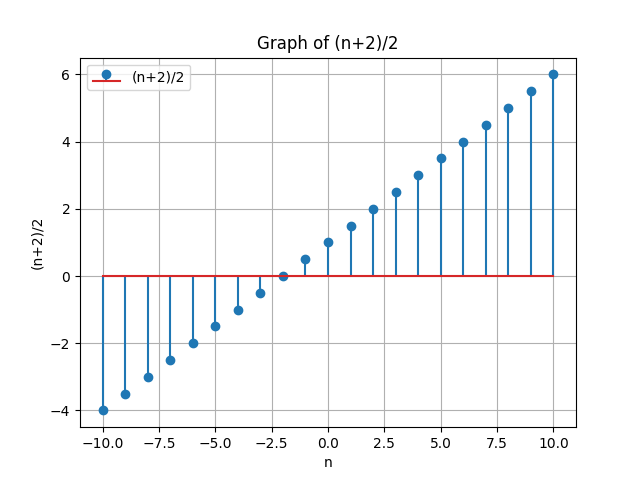
\includegraphics[scale=0.65]{py_3.png}
    %github/psrikarvarma/ss-assignment_1-jan2024/blob/main/discrete_progressions/figs/py_3.png
    \caption{Graph of $\left(\frac{n+2}{2}\right)$}
    \label{fig:enter-label}
\end{figure}\\
\begin{figure}
    \centering
    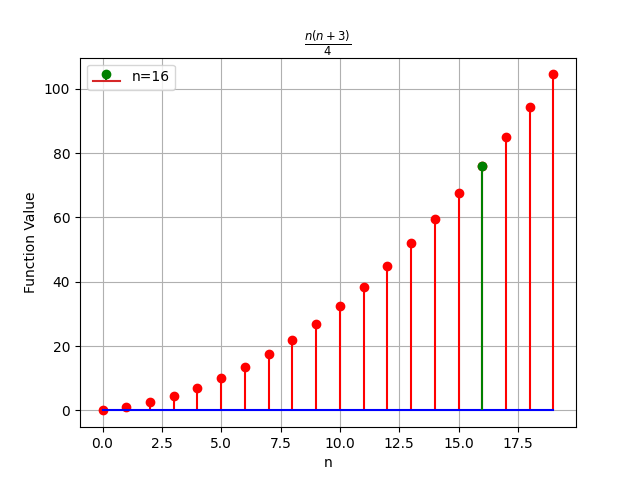
\includegraphics[scale=0.65]{py_4.png}
    %github/psrikarvarma/ss-assignment_1-jan2024/blob/main/discrete_progressions/figs/py_4.png
    \caption{Graph of $\left(\frac{n.(n+3)}{4}\right)$}
    \label{fig:enter-label}
\end{figure}\\
\begin{figure}
    \centering
    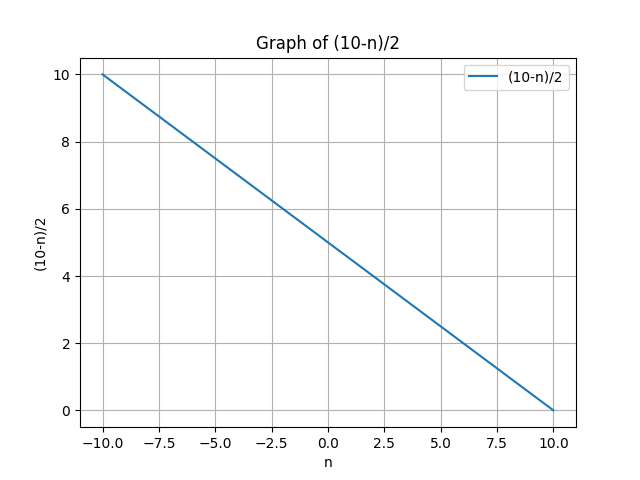
\includegraphics[scale=0.65]{py_5.png}
    %github/psrikarvarma/ss-assignment_1-jan2024/blob/main/discrete_progressions/figs/py_5.png
    \caption{Graph of $\left(\frac{10-n}{2}\right)$}
    \label{fig:enter-label}
\end{figure}\\\begin{figure}
    \centering
    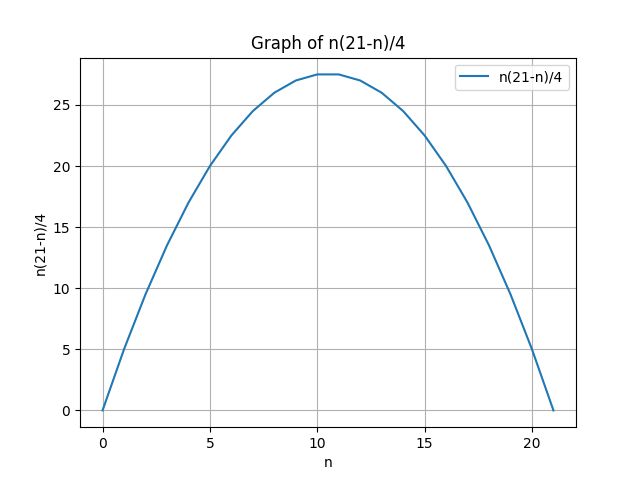
\includegraphics[scale=0.65]{py_6.png}
    %github/psrikarvarma/ss-assignment_1-jan2024/blob/main/discrete_progressions/figs/py_6.png
    \caption{Graph of $\left(\frac{n.(21-n)}{4}\right)$}
    \label{fig:enter-label}
\end{figure}

\end{document}
